\chapter{总结与展望}
本篇论文专注于量子转换系统的图像计算难题。呈现了一系列有效识别给定子空间基底的算法,并针对子空间及量子电路,提出了多种分割策略。还引入了预估子空间超集的算法,通过张量积基的集合进行表示。将这些要素融合,构建了多个算法,能够为量子系统的图像计算任务提供高效的解决方案。

在后续工作中,计划利用本研究的方法进行量子系统的模型检验,尤其关注那些可以通过时态逻辑表述的属性。也将深入探讨更为复杂系统的图像计算问题,特别是那些无法仅以量子电路形式表达的系统。

图像计算对于模型检验,无论是经典还是量子转换系统,都至关重要。本论文致力于通过介绍高效的图像计算算法,加速量子系统模型检验的进展。采用张量网络来表述量子电路,并利用张量网络及张量决策图的特性设计出高效的图像计算算法。经过实证评估证明,采用基于收缩分割的算法能大幅提升量子转换系统图像计算的效率。

本研究对量子系统的验证工作做出了重要贡献,在量子硬件与软件快速发展的大背景下,满足了对有效验证技术不断增长的需求。

展望未来,意图将本方法应用于量子系统的模型检验工作,尤其是在验证时态逻辑描述的属性方面。同时,也计划将图像计算拓展到更加复杂,不能仅通过量子电路表达的系统。这些研究将促进量子系统验证方法的理解和应用。
\section{论文总结}
量子模型检测是验证量子系统可靠性的一种自动化方法。
其面临的主要困难是随着量子系统中量子比特增加,资源需求指数增长。

在本次研究中,通过应用新的数据结构,TDD,试图降低资源消耗。并在
\section{工作展望}
在技术实现上,构建了两个版本的量子线路转化为TDD的工具,分别基于C语言和Python语言。这些工具的开发对于实现的研究方法至关重要,提高了实验的灵活性和效率。
其中的C语言的TDD支持任意维度张量,例如对双比特CNOT门,既可以按图\ref{fig:cnot-4}中的张量维度为4,
即按照索引为$q_1,q_0$进行表示。也可以按图\ref{fig:cnot-2}中的张量维度为4,
即按照索引为$q_3,q_2,q_1,q_0$进行表示。这样的设计大大提高了TDD的表示能力,为更复杂系统的验证提供了基础。
\begin{figure}[!htbp]
    \centering
    \begin{subfigure}[b]{.4\textwidth}
        \centering
        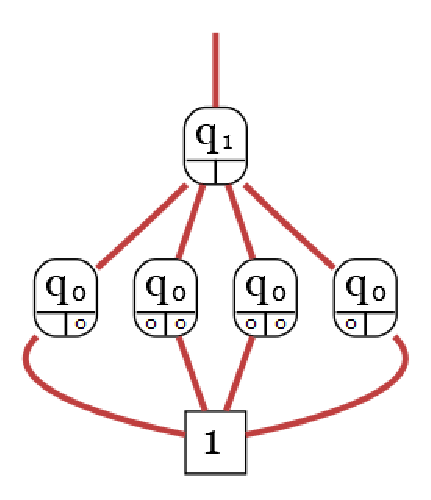
\includegraphics[height = 6cm]{Img/cnot.eps}
        \caption{张量维度为4的CNOT门的TDD表示}
        \label{fig:cnot-4}
    \end{subfigure}
    \begin{subfigure}[b]{.4\textwidth}
        \centering
        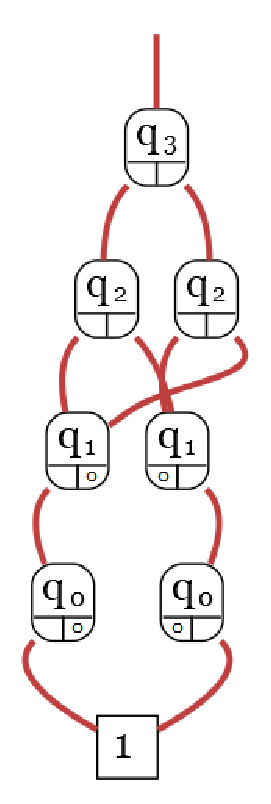
\includegraphics[height=6cm]{Img/cx.eps}
        \caption{张量维度为2的CNOT门的TDD表示}
        \label{fig:cnot-2}
    \end{subfigure}
    \caption{C语言版的TDD支持任意维度的例子}
    \label{fig-cnot}
\end{figure}
% //TODO: add limdd data
\subsection*{limdd的改进}
由于量子状态都在同一希尔伯特空间中。因此作用某些算子后,不同的量子状态可能等价。
当存储算子的资源少于存储状态的资源时,就有可能存储算子表示不同的状态\citep{vinkhuijzen2023limdd}。图\ref{fig:qmdd-example}表示了一个QMDD的例子,应用等价性,可以化简为图\ref{fig:limdd-example}。
TDD也可以应用类似技术,进行进一步化简,从而降低资源要求。
\begin{figure}[!htbp]
    \centering
    \begin{subfigure}[b]{.4\textwidth}
        \centering
        \includegraphics[height=8cm]{Img/limdd.pdf}
        \caption{一个QMDD示例}
        \label{fig:qmdd-example}
    \end{subfigure}
    \begin{subfigure}[b]{.4\textwidth}
        \centering
        \includegraphics[height=8cm]{Img/limdd_reduce.pdf}
        \caption{应用等价性化简图\ref{fig:qmdd-example}}
        \label{fig:limdd-example}
    \end{subfigure}
\end{figure}
% //TODO:add here
\textcolor{red}{limdd的原理}